% id: 0079
% book: RPM 공통수학1 · 01 다항식의 연산
% section: 유형 12 조립제법
% figure: crop:fig-0079.png
% answer: $19$
% answer_source: 답지
% variant_level: 0 (원본 전사)
% 이 파일은 build.mjs 가 items.json 에서 만든다. 고칠 때는 items.json 을 고친다.
\smash{\raisebox{1.5mm}{\dmkichul{RPM 공통수학1 0079번 · 15쪽 · 대표문제}}}
\noindent\begin{minipage}[t]{0.58\linewidth}\vspace{0pt}\raggedright 오른쪽은 다항식 $3x^3-2x^2-5x+1$을 $x-2$로 나누었을 때의 몫과 나머지를 조립제법을 이용하여 구하는 과정이다. 이때 $a+b+R$의 값을 구하시오.\end{minipage}\hfill\begin{minipage}[t]{0.4\linewidth}\vspace{0pt}\centering 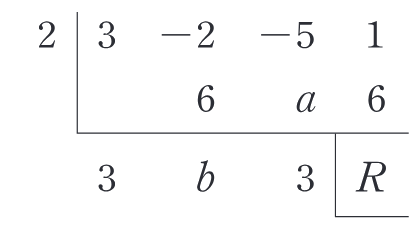
\includegraphics[width=99.9pt]{figures/fig-0079.png}\end{minipage}\par
